\documentclass[10pt, xcolor=dvipsnames]{beamer}

\usetheme{metropolis}
\usepackage[utf8]{inputenc}
\usepackage[english]{babel}
\usepackage{ragged2e}
\usepackage{bbding}
%\usepackage{enumitem}
\usepackage{mathtools}
\usepackage{indentfirst}
\usepackage{graphicx}
\usepackage{float}
\usepackage{hyperref}
\usepackage{mathtools}
\usepackage{preview}
\usepackage{xcolor}
\usepackage{color}
\usepackage{listings}
\usepackage{float}
\usepackage[caption = false]{subfig}
\usepackage{pdfpages}
\usepackage{multirow}
\usepackage{array}
\usepackage{makecell}
\usepackage{bm}
\usepackage{caption}
\usepackage{cancel}
\usepackage{anyfontsize}
\usepackage{etoolbox}
\usepackage{mathtools}

\usepackage[flushleft]{threeparttable}
\usepackage{booktabs}
\usepackage{caption}
\usepackage{adjustbox}
\usepackage{appendixnumberbeamer}
\usepackage{pifont}
\usepackage{amsmath}
\usepackage{amssymb}
\usepackage[percent]{overpic}

%\usepackage{biblatex}
\usepackage[backend=biber,
style=authoryear,
citestyle=authoryear]{biblatex} 
\addbibresource{latex/bibliography.bib}

\setbeamercolor{titlelike}{parent=structure}
\definecolor{UBCblue}{rgb}{0.04706, 0.13725, 0.32}
\colorlet{UBCblue2}{UBCblue!70!white}
\usecolortheme[named=UBCblue]{structure}

\makeatletter
\setbeamertemplate{footline}
{
  \leavevmode%
  \hbox{%
  \begin{beamercolorbox}[wd=.4\paperwidth,ht=2.25ex,dp=1ex,center]{author in head/foot}%
    \usebeamerfont{author in head/foot} \insertshortauthor %\hspace*{1em}(\insertshortinstitute)
  \end{beamercolorbox}%
  \begin{beamercolorbox}[wd=.5\paperwidth,ht=2.25ex,dp=1ex,center]{title in head/foot}%
    \usebeamerfont{title in head/foot} \insertshorttitle
  \end{beamercolorbox}%
  \begin{beamercolorbox}[wd=.1\paperwidth,ht=2.25ex,dp=1ex,center]{date in head/foot}%
    \usebeamerfont{date in head/foot}
    \insertframenumber{} / \inserttotalframenumber\hspace*{2ex} 
  \end{beamercolorbox}}%
  \vskip0pt%
}
\makeatother

\renewcommand{\arraystretch}{1.2}
\renewcommand{\raggedright}{\leftskip=0pt \rightskip=0pt plus 0cm}
\newcolumntype{C}[1]{>{\centering\let\newline\\\arraybackslash\hspace{0pt}}m{#1}}

\hypersetup{
    colorlinks=true,
    linkcolor=UBCblue,
    citecolor=UBCblue,
    filecolor=magenta,      
    urlcolor=blue,
    allcolors=.
}

\setbeamercolor{button}{bg=UBCblue2,fg=white}
\newcommand\fnote[1]{\captionsetup{font=tiny}\caption*{#1}}
\newcommand\fnotev[1]{\captionsetup{font=scriptsize}\caption*{#1}}
\def\house{\hbox{\kern3pt \vbox to13pt{}% 
   \pdfliteral{q 0 0 m 0 5 l 5 10 l 10 5 l 10 0 l 7 0 l 7 5 l 3 5 l 3 0 l f
               1 j 1 J -2 5 m 5 12 l 12 5 l S Q }%
   \kern 13pt}}
\setbeamertemplate{caption}[numbered]
\setbeamertemplate{itemize item}{\Tiny \house}
% %\justifying
% \urlstyle{same}
%\usefonttheme{serif}

%------------------------
%------------------------

\date{}

%------------------------
%------------------------
%----------------------------------------------------------------------------------------
%	TITLE PAGE
%----------------------------------------------------------------------------------------------------------------
%------------------------

\title[Joe Fish Prospectus]{How Should We Think About Low Income Rental Markets} % The short title appears at the bottom of every slide, the full title is only on the title page
\author[Joe Fish]{Joe Fish}


\begin{document}

\begin{frame}
\titlepage % Print the title page as the first slide
\end{frame}

\begin{frame}{Dissertation Chapters}
    \begin{enumerate}
        \item A search model of the low income rental market (job market paper)
        \item Landlord Responses to Changes in Tenant Protections
        \item Are Large Investors A Source of Declining Rental Affordability: Evidence from Boston, MA and Houston, TX (field paper)
    \end{enumerate}
    
\end{frame}

\section{Field Paper}

\begin{frame}{Recap of Field Paper}
    \textbf{Big Picture:} \textcolor{blue}{How should we think about large landlords?}\\
    \pause
    \vspace{0.5cm}
    \textbf{Case study of two rental markets (Boston and Houston)}
    \begin{enumerate}
        \item What are long term trends in rental markets?
        \begin{itemize}
            \item Is concentration increasing?
            \item What kinds of properties do different landlords target?
        \end{itemize}
        \pause
        \item When landlords buy properties, what do they do to rent prices? 
        \begin{itemize}
            \item Are price effects related to landlord characteristics?
        \end{itemize}
        \pause
        \item What are the economics that rationalize acquisition effects?
        \begin{itemize}
            \item market power, information asymetry, renovations, etc.
        \end{itemize}
    \end{enumerate}
\end{frame}

\begin{frame}{Recap of Field Paper: Results}
    \begin{itemize}
    \item First, I show that failing to take into account shell ownership leads to underestimates of market concentration of more than 10\%.
    \pause
    \item Second, I show that, while shell ownership matters for accurately measuring levels of concentration, I find no evidence that concentration has increased over time.
    \pause
    \item Third, I show that over 90\% of the variation in concentration within a market across time is explained by entry, and only 5\% by mergers.
    \pause
    \item Fourth, I find that, on average, landlords raise prices by 1.7 percentage points after acquiring properties (over 4 percentage points by the fourth year post-acquisition).
    \pause
    \item Fifth, I show that these acquisition effects are largely explained by post-acquisition renovations. Specifically, I estimate precise null effects for properties that are acquired but not subsequently renovated and large effects for those that are subsequently renovated.
  \end{itemize}
    
\end{frame}

\section{Job Market Paper: The Economics of Low Income Rental Markets}

\begin{frame}{Motivation}
    \begin{enumerate}
        \item About 80\% of low income renters live in private market units \parencite{jchs_2024, nhpd2024profiles}
        \pause
        \item Low income landlords are both more punitive (lower threshold to evict) and more profitable \parencite{Desmond_2019, Eisfeldt_2015,Damen_2025}
        \item Evictions have large personal and social cost \parencite{desmond-evicted,humphries2025, collison-et-al-2023}
        \begin{itemize}
            \item Suggests room to regulate the worst landlords
        \end{itemize}
        \pause
        \item At the same time, given reliance on private market and lack of funds for subsidized housing, optimal regulation has to be careful about inducing landlord exit
        \begin{itemize}
            \item Ex ante unclear what optimal regulation looks like, but optimal regulation requries knowing \textbf{extent and sources of market power} and \textbf{landlord exit options}
        \end{itemize}
    \end{enumerate}

\end{frame}

\begin{frame}{Research questions}

\begin{enumerate}
    \item \textbf{Is search and matching the correct way to think about rental market power?}
    \begin{itemize}
        \item More specifically, what do we get wrong if we ignore bargaining and search frictions?
    \end{itemize}
    \pause
    \item What do the exit decisions of low income landlords look like? Specifically, who are the \textbf{marginal} vs \textbf{inframarginal} landlords
    \pause
    \item Given knowledge of landlord markups and exit decisions, what's the best way to regulate the low income rental market?
\end{enumerate}

\end{frame}

\begin{frame}{This Presentation}
    \begin{enumerate}
        \item Present stylized facts about the Philadelphia Rental Market
        \begin{itemize}
            \item high prices consistent with prior literature
            \item evidence of market segmentation
        \end{itemize}
         \pause
        \item \cite{jarosh-search-2024} search model adapted to the rental market
        \pause
        \begin{itemize}
            \item Key intuition: Rental market looks more like the labor market than a generic product market $\rightarrow$ search frictions and bargaining are going to be a large source of market power
            \item In particular, large landlords likely have some lattitude to affect tenants' consideration sets
        \end{itemize}
    \end{enumerate}
    
\end{frame}

% \begin{frame}{Contributions}

% \begin{itemize}
%     \item One of the first datasets to have a comprehensive and representative unit-level rent panel of a major American rental market
%     \item 
%     \item First paper to provide landlord exit thresholds 
% \end{itemize}
    
% \end{frame}

\begin{frame}{Literature on Evictions and Low-Income Landlords}
    \textbf{Prices and Profits}
        \begin{itemize}
                \item Low Income landlords have \textbf{higher} profit margins than any other kind of landlord \parencite{Desmond_2019, Damen_2025, Eisfeldt_2015}
                \item Rent Prices are often as high as they are in much higher quality neighborhoods; maintenance is much lower 
        \end{itemize}
    \pause 
    \textbf{Landlord Business Models}
    \begin{itemize}
        \item ~9\% of rent goes unpaid \parencite{collinson2024eviction} and about 8\% of tenants have an eviction filed against them per year in Philadelphia (4\% eviction rate)
        \item Landlords allow about two months of back rent before filing to evict (\cite{humphries-2024} and Author's calculations)
        \begin{itemize}
            \item Intuition for why landlords wait: A large fraction of tenants default and then repay, so it's optimal for landlords to learn about tenant's probability of repayment
        \end{itemize}
    \end{itemize}
    
\end{frame}

\begin{frame}{Literature on Rental Markets}
    Rental markets are understudied because of poor data availability\\
    \vspace{0.25cm}
    \begin{itemize}
        \item Recently (last ~5 years) private rental data has made granular studies of the rental market feasible
        \begin{itemize}
            \item \cite{calderwang2024algorithmic} on algorithmic pricing, \cite{framoutar2024market} on rental market monopoly power, and \cite{gurun-et-al-2022} on institutal landlords as examples
        \end{itemize}
        \item However, these private data overwhelmingly sample from the formal, professionally managed, and higher income sectors
        \item My paper will be one of the only to have unit level data on the low income rental market
        \begin{itemize}
            \item \cite{humphries-2024}, which has lease ledger data for a large low income landlord a notable exception
        \end{itemize}
    \end{itemize}
\end{frame}

% \begin{frame}{Literature On Landlord Market Power}
% TBD
    
% \end{frame}


\section{Data}

\begin{frame}{Data and Institutional Setting}
\textbf{Philadelphia}
    \begin{itemize}
        \item Universe of Eviction Records from 2006-2019
        \begin{itemize}
            \item Contain \textbf{contract rents} as well case information (address, amount owed, plaintiff / defendant name, etc.)
            \item Cases are filtered to non-commercial and non-housing authority
        \end{itemize}
        \item Rental listing data from Altos (2011-2019)
        \begin{itemize}
            \item Unit level rental listings with information on amenities, beds, baths, etc. 
        \end{itemize}
        \item Rental Registry from 2016-2019 (covers about 90\% of rental units in Philadelphia)
    \end{itemize}
    \pause
    Why this is important:\\
    \begin{itemize}
        \item This will be one of the few papers to study the low income rental market because data are so sparse 
    \end{itemize}
\end{frame}

\begin{frame}{Distribution of Rent Prices by Data Source}
Commercially available rental datasets (\textcolor{red}{altos}) don't cover the low income rental market\\
    \begin{figure}
        \centering
        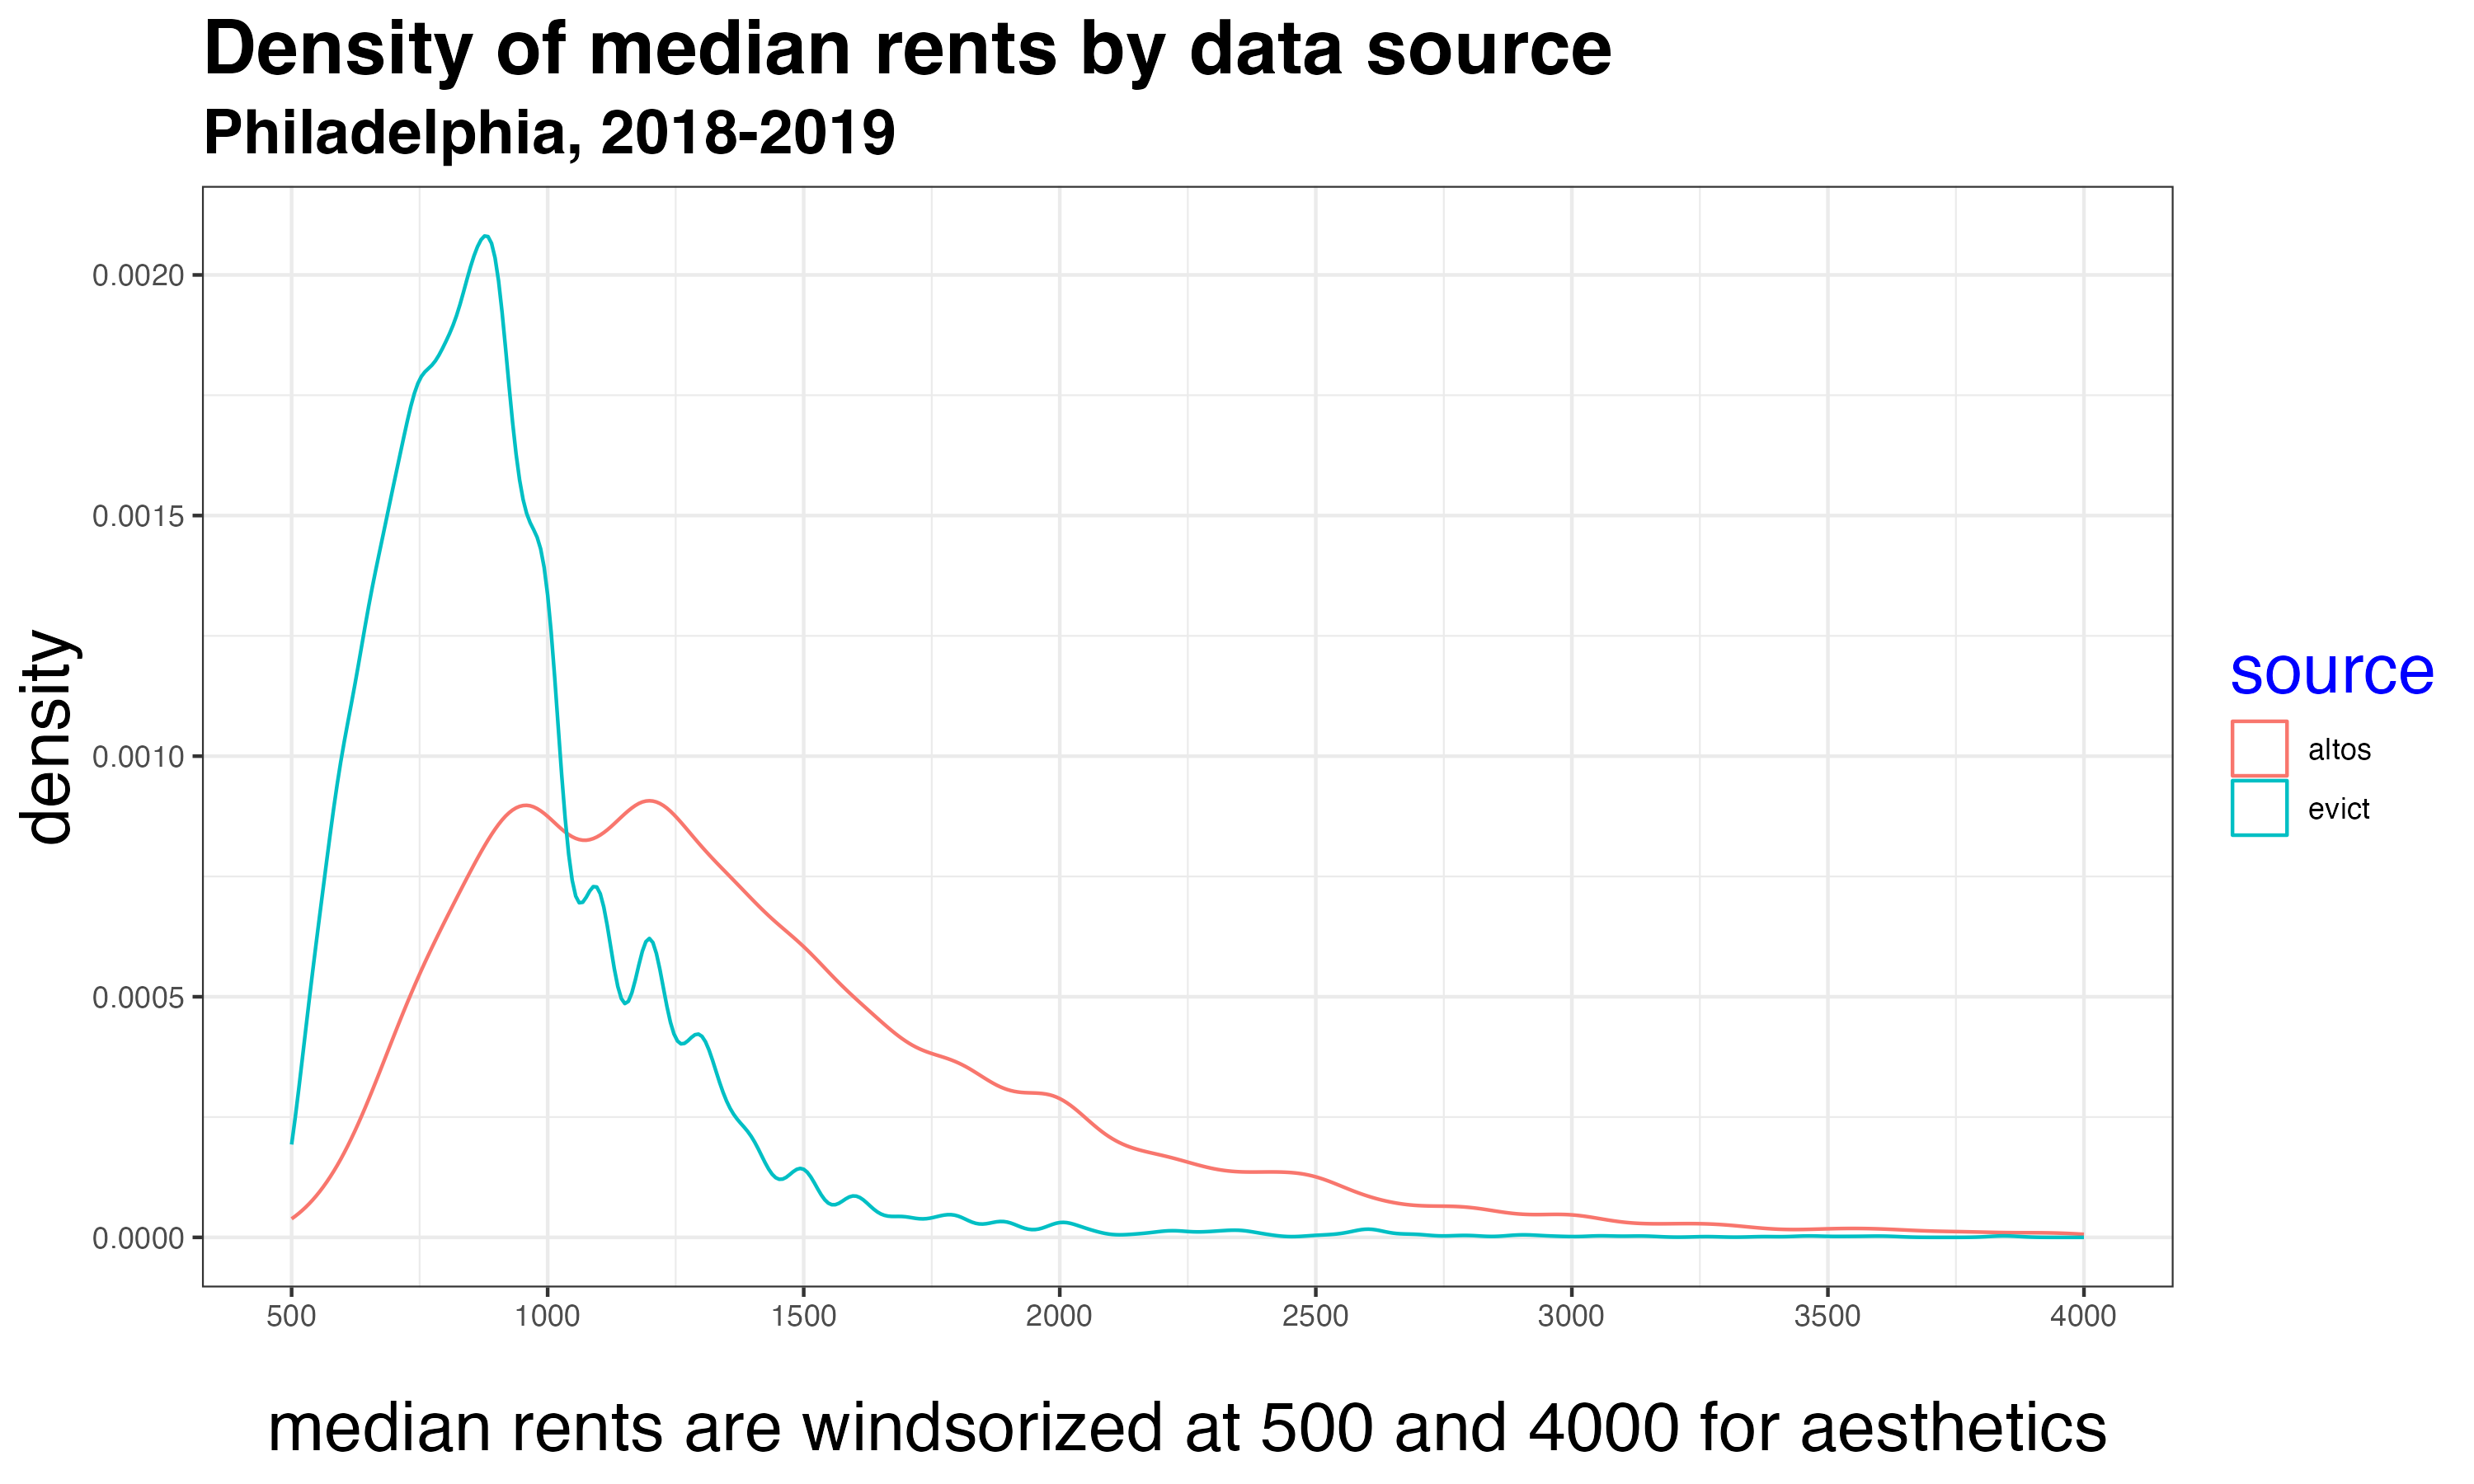
\includegraphics[width=0.75\linewidth]{figs/density_rent_prices.png}
        \caption{Rent Prices by Data Source}
        \label{fig:rent-dist}
    \end{figure}
\end{frame}




\section{Stylized Facts}

\begin{frame}{Stylized Facts}
    \begin{enumerate}
        \item Hedonic Regressions suggest prices for high evicting rental units are higher than what we'd expect, given observable quality
        \item Rental Markters are generally not consolidated, however, the low income rental market likely is -- largely due to the limited number of landlords who will rent to tenants with eviction histories and poor credit
        \item I take 1) and 2) as suggestive evidence of landlord market power
    \end{enumerate}
\end{frame}

% \begin{frame}{Eviction in Low Income Rental Markets}
% \textbf{Eviction}
%     \begin{itemize}
%         \item Eviction is common: (~8-25 evictions / 100 renter households / year)
%         \item ~9\% of rent goes unpaid
%         \item Landlords allow about two months of back rent before filing to evict
%         \begin{itemize}
%             \item Intuition is a large fraction of tenants default and then repay; landlords learn about tenant's probability of repayment
%         \end{itemize}
%         \item Landlords anecdotally say they collect \$.10 for every \$1 in money judgment 
%         \item Most low income tenants rent from the private market
%         \begin{itemize}
%             \item ~20 million severely rent burdened households and about ~5 million subsidized housing units
%         \end{itemize}
%     \end{itemize}
%     \pause
    
% \end{frame}

\begin{frame}{Prices in Low Income Rental Markets}
\textbf{Hedonic Regressions}
    \begin{itemize}
    \item Intuitively, we should expect high filing rates (average number of evictions per unit per year) to be negatively correlated with rents
    \begin{itemize}
        \item High eviction rates may signal unobserved quality
        \item High eviction rates may signal lower threshold to evict
    \end{itemize}
    \pause
        \item Unconditionally, eviction rates don't correlate with prices after a ~20\% filing rate
        \pause
        \item After controlling for property and neighborhood characteristics, units with \textbf{higher} eviction rates charge \textbf{higher} rents 
    \end{itemize}
\end{frame}

\begin{frame}{Bin Scatter Eviction Rates vs Rents}
    \begin{figure}
        \centering
        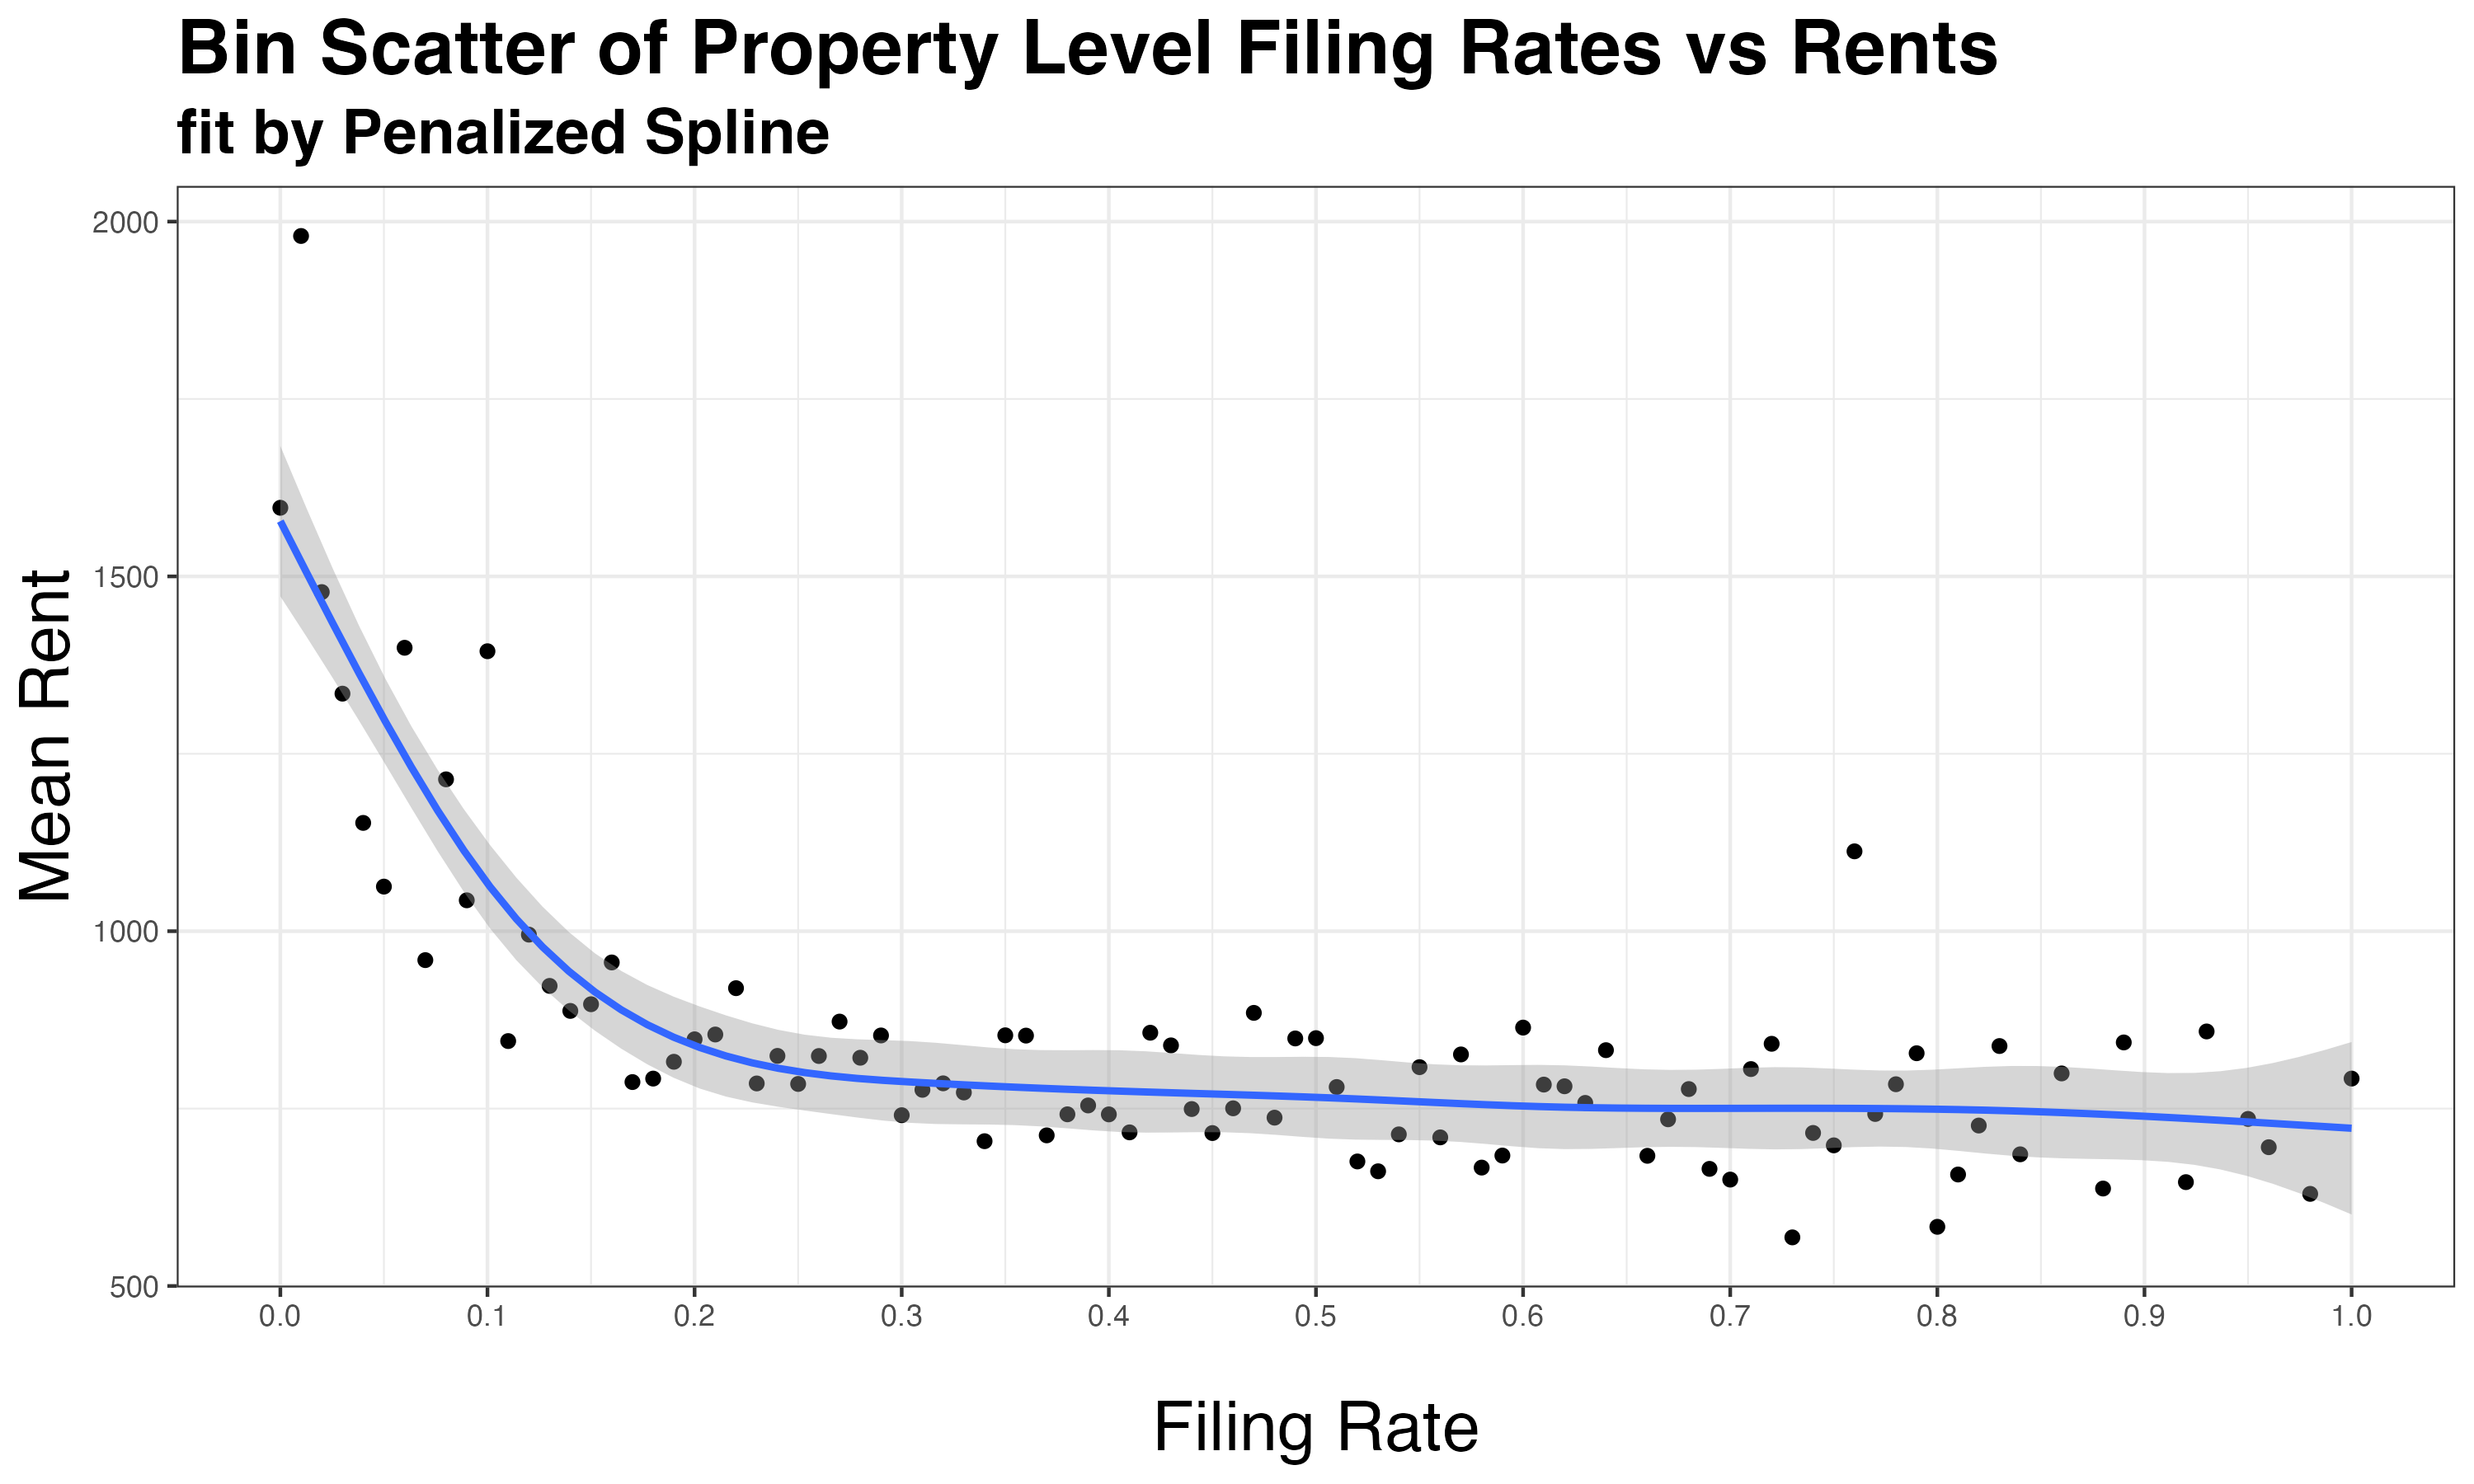
\includegraphics[width=0.75\linewidth]{figs/philadelphia_filing_rate_rent_scatter.png}
        \caption{Bin Scatter of Eviction Rates by Data Source}
        \label{fig:bin-scatter}
    \end{figure}
\end{frame}

\begin{frame}{Hedonic Regressions of Rent Prices}
    \begin{center}
    \Tiny
        \begin{table}[htbp]
   \caption{\label{tab:rent_regs} Rent Price Regressions}
   \centering
   \begin{tabular}{lcc}
      \tabularnewline \midrule \midrule
      Dependent Variable: & \multicolumn{2}{c}{Log(Price)}\\
      Model:                       & (1)             & (2)\\  
      \midrule
      \emph{Variables}\\
      Filing Rate                  & -0.9082$^{***}$ & 0.0122$^{**}$\\   
                                   & (0.0888)        & (0.0054)\\   
      Polynomial Imputed Beds      & No              & Yes\\  
      Polynomial Imputed Baths     & No              & Yes\\  
      Polynomial Year Built        & No              & Yes\\  
      Polynomial Number of Stories & No              & Yes\\  
      Polynomial Number of Units   & No              & Yes\\  
      \midrule
      \emph{Fixed-effects}\\
      Year                         & Yes             & \\  
      Census Block Group-Year      &                 & Yes\\  
      Heater Type                  &                 & Yes\\  
      Quality Grade                &                 & Yes\\  
      View Type                    &                 & Yes\\  
      Building Code                &                 & Yes\\  
      Construction Type            &                 & Yes\\  
      \midrule
      \emph{Fit statistics}\\
      Observations                 & 55,848          & 54,315\\  
      R$^2$                        & 0.25091         & 0.84653\\  
      \midrule \midrule
      \multicolumn{3}{l}{\emph{Clustered (Parcel ID) standard-errors in parentheses}}\\
      \multicolumn{3}{l}{\emph{Signif. Codes: ***: 0.01, **: 0.05, *: 0.1}}\\
   \end{tabular}
\end{table}

    \end{center}
\end{frame}

% \begin{frame}{Explanations for High Prices}
%     \begin{itemize}
%         \item High prices reflect high default risk
%         \begin{itemize}
%             \item Definitely true, but can't rationalize higher \textbf{profits} shown in related literature
%         \end{itemize}
%     \end{itemize}
    
% \end{frame}

\begin{frame}{Market Segmentation in Low Income Rental Markets}
    \begin{itemize}
        \item There's qualitative evidence that tenants with eviction histories have trouble renting housing \parencite{desmond-evicted}
        \pause
        \item In the future, I'd like to use address history data to empirically document substitution patterns for renters with eviction histories
        \pause
        \item Until then, I segment markets based on zip code and property type, following \parencite{framoutar2024market, calderwang2024algorithmic} and by whether the unit had an above 15\% average filing rate
        \pause
        \item I'll show that, if you think because of tenant screening, low income renters substitute largely between high evicting properties, markets can be fairly consolidated
    \end{itemize}
\end{frame}

\begin{frame}{Market Segmentation in Low Income Rental Markets}
    \begin{itemize}
        \item The typical renter rents from a landlord who owns a negligble share of their market's units
        \item Many \textbf{low income} renters rent from a landlord who owns a substantial share of their market's units
    \end{itemize}
    \begin{figure}
        \centering
        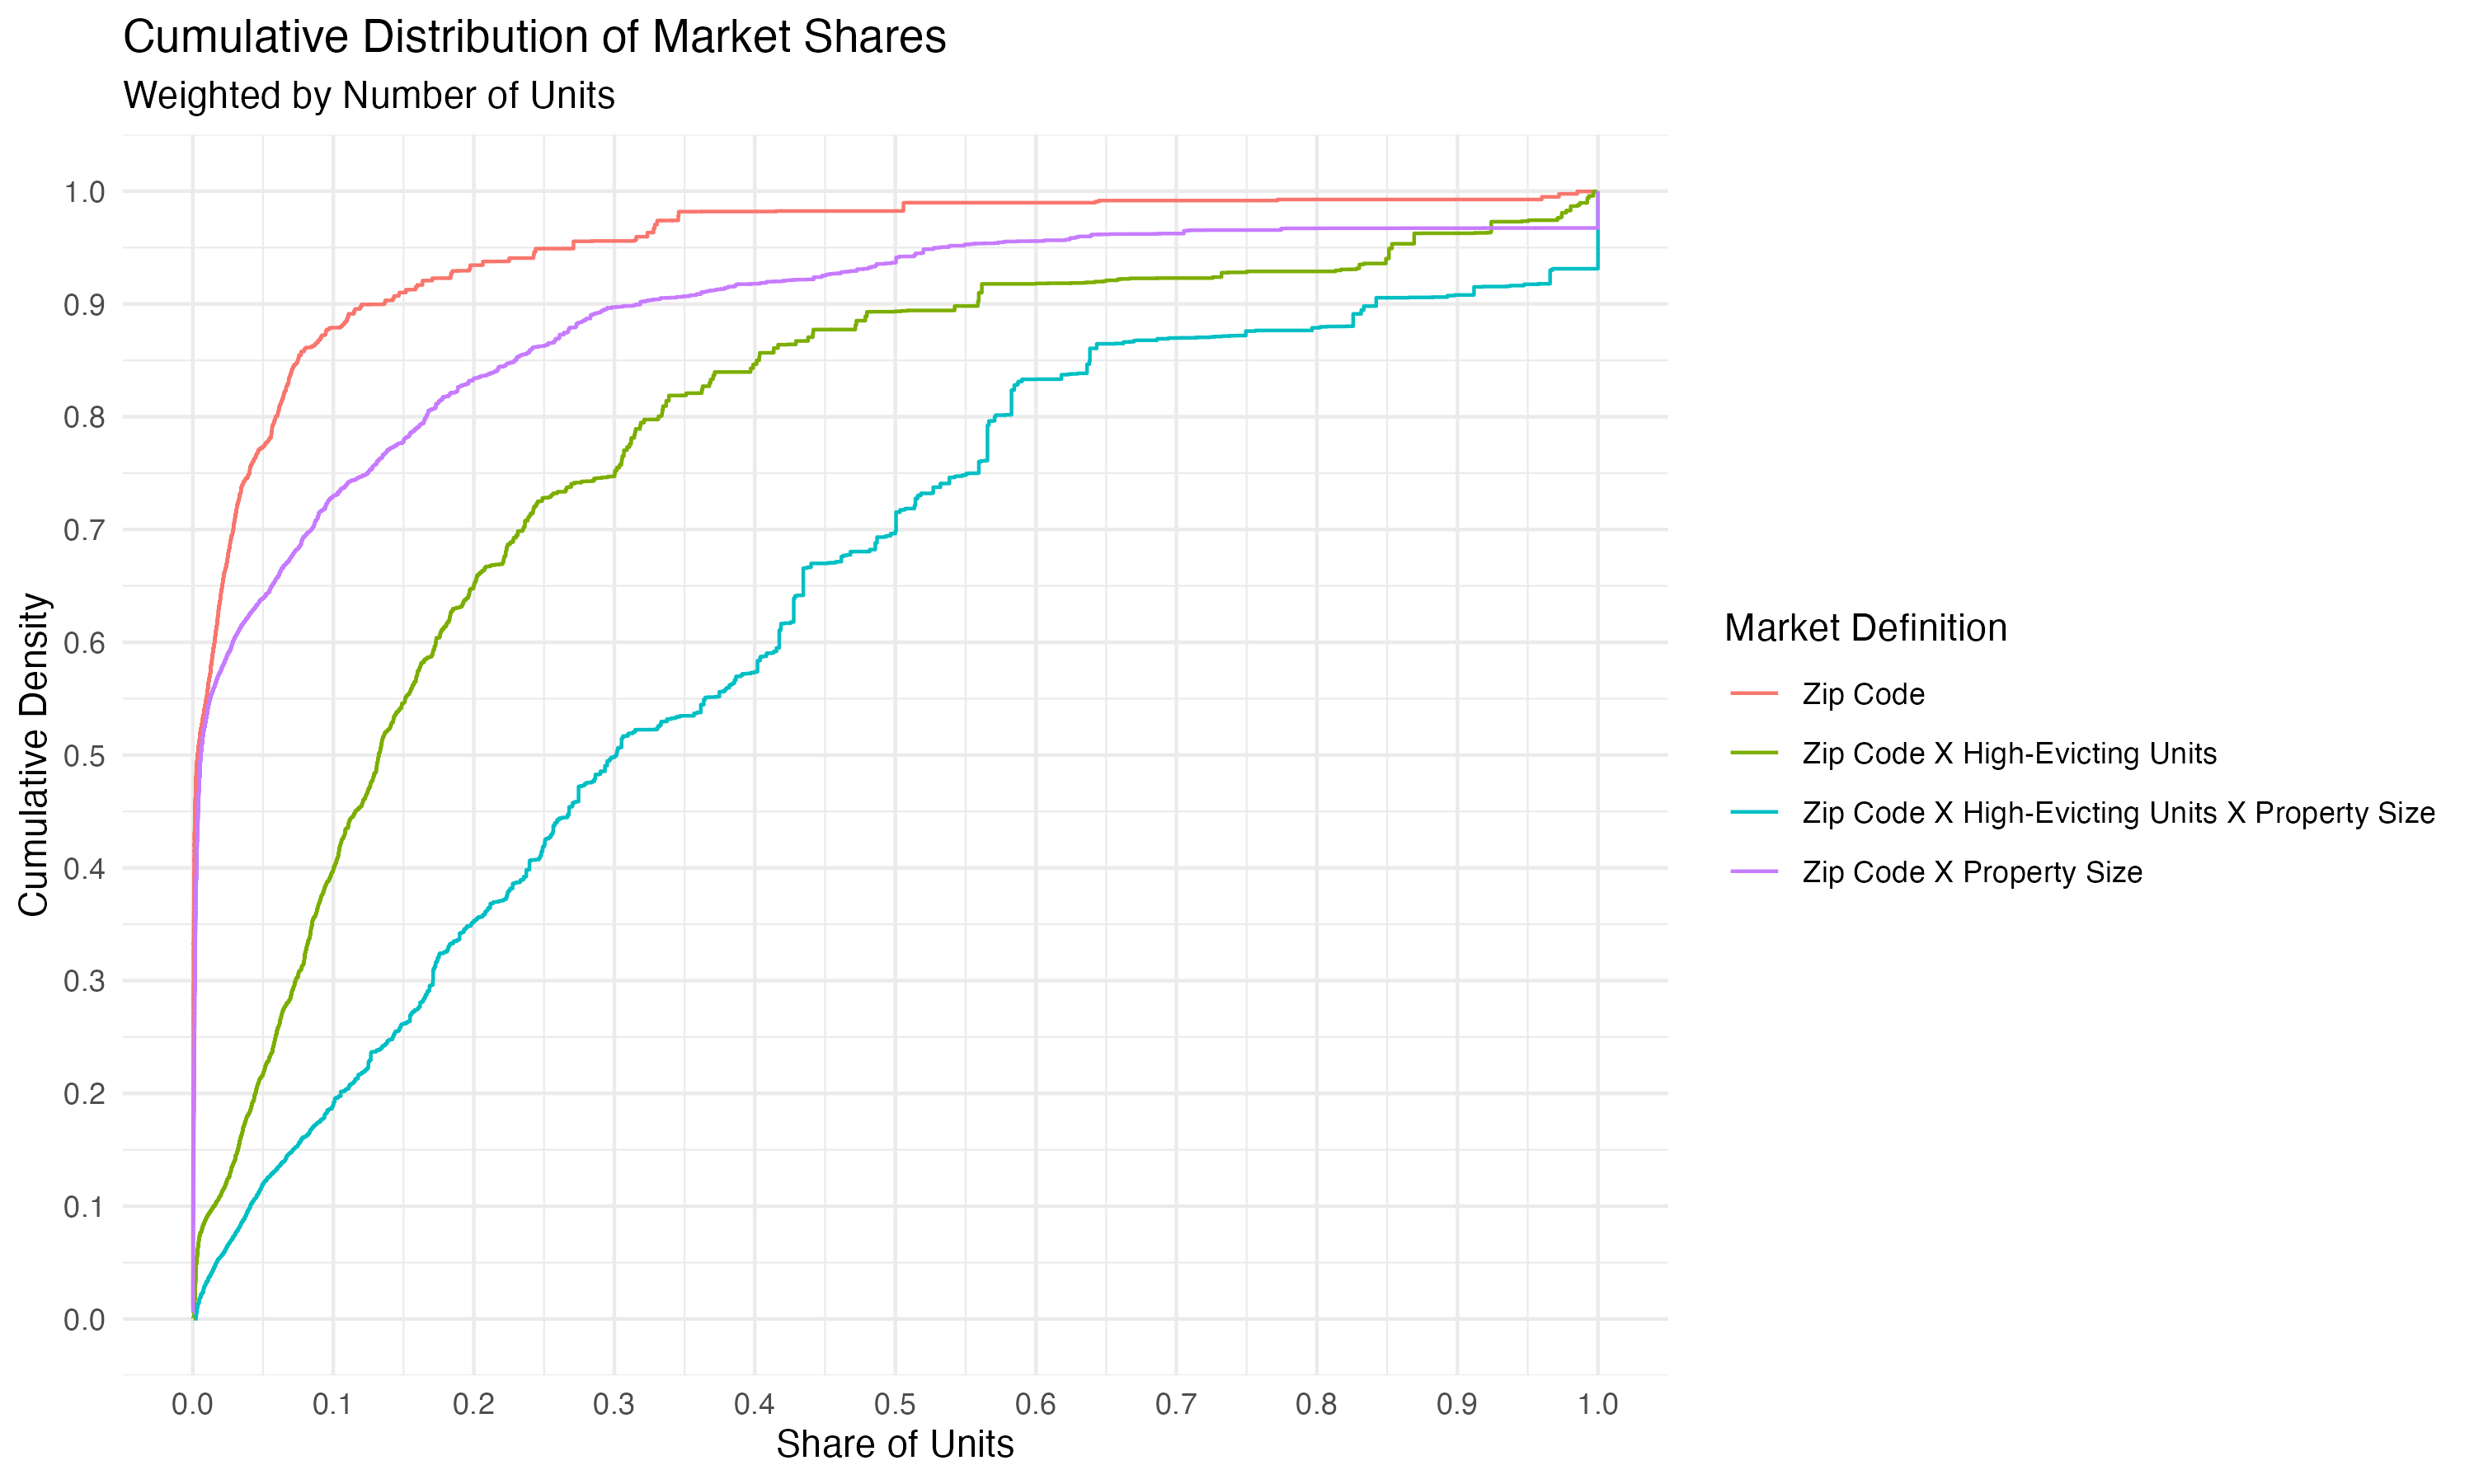
\includegraphics[width=0.75\linewidth]{figs/market_share_cdf.png}
        %\caption{Caption}
        \label{fig:market-share-cdf}
    \end{figure}
\end{frame}

% \begin{frame}{Share Regressions}
    
% \end{frame}


% \begin{frame}{Rationalizing High Prices}
% \textbf{Default Premia can explain higher prices but not higher profits}, implies need to model market power
%     \begin{itemize}
%     \item Most models of rental market power assume competition is differentiated products bertrand \parencite{watson2024rent, framoutar2024market}
%         \item Landlords flex market power with product differentiation and \textbf{quantity restriction}
%         \item Market structure matters to the extent it influences landlords' \textbf{residual demand curves}
%     \end{itemize}

% \end{frame}

\begin{frame}{Motivating the Search Model}\label{slide:searchmotivation}
The rental market looks more like the labor market than a standard product market:\\
    \begin{itemize}
        \item Landlords (firms) post vacancies
        \item Tenants (workers) search for homes (jobs) and apply
        \begin{itemize}
            \item Many vacancies get multiple applicants, so tenants have guarantee that they can rent a particular vacant unit
        \end{itemize}
        \item Housing has to be consumed every period or households are forced into outside option (unemployment analogy)
        \item Prices have a certain degree of bargaining
    \end{itemize}

    \hyperlink{slide:fern-prices}{\beamergotobutton{Empirics }}
    
\end{frame}

\begin{frame}{The slide that I wish I had}

\begin{itemize}
    \item The paper would be much stronger if I had a slide showing exactly what researchers would get wrong if they didn't put search frictions and bargaining into their models.
    \item Currently, the closest I have are some other papers' reduced form estimations of the effects of mergers, which can't easily be rationalized by post-merger quantity restriction
    \item Lastly, I love the intuition and economics behind the search model, but I think the paper would be stronger if the model could be blended with more traditional demand estimation
\end{itemize}
    
\end{frame}

% \begin{frame}{Models of Landlord Market power}

    
% \end{frame}

\begin{frame}{Search Model}
\cite{jarosh-search-2024} labor search model, adapted for the rental market 
    \begin{itemize}
        \item Standard search and matching model for labor
        \item Twist is that landlords can remove themselves from tenants' outside option
        \begin{itemize}
            \item Intuition is landlords can say "you can rent this unit, but if you refuse my offer, I won't show you any other units"
            \item This is costless in world where vacancies see multiple applications
        \end{itemize}
        \item Model delivers market power without landlords having to reduce vacancies
    \end{itemize}
\end{frame}

\begin{frame}{Model Setup}
    \begin{itemize}
    \item Discrete time economy
    \item Unit measure of infinitely lived, homogenous renters
    \item Renters are either housed and pay rent ($r$) to receive flow utility (\textbf{$\eta$}) or are unhoused / consuming some outside housing good \textbf{$u$} and searching while receiving flow utility \textbf{$b$}
    \item Common discount factor \textbf{$0 < \beta < 1$}
    \item Housed / non-searching renters experience exogenous separation shock at rate \textbf{$\delta$}
\end{itemize}
\end{frame}

\begin{frame}{Matching}
    \begin{itemize}
    \item For each rental vacancy, landlords pay a per period cost of \textbf{$c_i$}
    \item Urn-ball matching function. Each period, \textbf{$u$} unhoused tenants send one application (balls) towards \textbf{$v$} vacancies (urns).
    \begin{itemize}
        \item Due to coordination frictions, some vacancies see $>1$ applications and some see zero. Applications per vacancy are exponentially distributed
    \end{itemize}
    \item If a landlord gets multiple applicants, they select one at random to follow up with and Nash bargain over rents
    % \begin{itemize}
    %     \item Nash bargaining; $0 \leq \alpha \leq 1$
    %     \item In this model, landlords aren't allowed to have applicants bid up the rents (unclear why this couldn't be allowed, but I don't do it here)
        
    % \end{itemize}
    \item Tenants are assumed to search randomly within a market (equivalent to vacancies appearing randomly); no directed search.
    \item Home finding rate = \textbf{$\lambda \equiv \frac{v}{u}(1-e^{-\frac{v}{u}})$}
\end{itemize}
\end{frame}

\begin{frame}{Tenant Value Functions}
\begin{itemize}
    \item \textbf{U} = value of outside option (homelessness; living in non-preferred neighborhood); \textbf{R} = rent paid; \textbf{b} = flow utility of outside option; \textbf{$\eta$} = flow utility of housing
    \item \textbf{$f_i$} indicates landlord size (market share)
    \item \begin{equation}
        U = b + \beta\left(\lambda \sum_{i} f_i(\eta - R_i) + (1-\lambda)U\right)\label{eq:tenant-val}
    \end{equation}
    \item Value of outside option is equal to flow utility plus probability of being housed in next period times the value of being housed plus the probability of remaining unhoused times the value of being unhoused
\end{itemize}
\end{frame}

\begin{frame}{Threat and Market Power}
    \begin{itemize}
    \item In eq \ref{eq:tenant-val}, landlords compete with themselves because the landlord's other vacancies enter the tenant's outside option
    \item What landlords can do instead is (partially) remove themselves from the tenants' outside option by committing themselves to not renting to the tenant in the future in the event bargaining breaks down.
    % \begin{itemize}
    %     \item This commitment works by landlord's choosing applicants randomly but removing the tenant in the event they have multiple applicants.
    %     \item Importantly, this is costless to the landlord, since they have multiple applicants. (If the deviating tenant is sole applicant, they get the unit)
    % \end{itemize}
    \item Here, I say that this punishment lasts until the tenant's search is over, so landlords need only be able to recognize a tenant's application for a short period of time
    % \begin{itemize}
    %     \item Intuitively, one could imagine a property manager making an take it or leave it offer to a tenant with the threat that if they leave it they can't see other units
    % \end{itemize}
    \end{itemize}
\end{frame}

\begin{frame}{Threat and Market Power Cont}
    \begin{itemize}
         \item Continuation value in event of breakdown:
        \item define \textbf{$\underline{\lambda}$} as the probability of being the sole applicant to a vacancy (in which case landlord will rationally accept applicant, even if punished)
        \begin{equation}\label{eq:match-val}
            U_i = b + \beta \left(\lambda\sum_{j\neq i}f_i(\eta - R_j) + \underline{\lambda} f_i(\eta - R_i) + (1-\lambda(1-f_i) - \underline{\lambda} f_i)U_i\right)
        \end{equation}
        \item first term is outside option, second term is probability of finding a vacancy at another landlord's unit, third term is probability of being the only applicant at the landlord's unit, and the fourth term is the probability of remaining unhoused
    \end{itemize}
\end{frame}

\begin{frame}{landlord Value Function}
    \begin{itemize}
    \item Value of match to landlord \begin{equation}
        J_i = R_i + \beta(1 - \delta)J_i
    \end{equation} 
    \item Value of match is equal to the rent paid + the discounted probability of continuing the match the following period 
    \item Value of landlord i of filling vacancy \begin{equation}\label{eq:job-value}
        V_i = -c_i + \beta(1  - e^{-\frac{u}{v}})J_i
    \end{equation}
    \begin{itemize}
        \item Value of vacancy is fixed cost plus probability landlord has at least one application; in equilibrium trade never breaks down and the match is always formed 
    \end{itemize}
    \item Joint surplus: \begin{equation}\label{eq:surplus-value}
        S_i \equiv (\eta - R_i) - U_i + J_i
    \end{equation}
    \end{itemize}
\end{frame}

\begin{frame}{landlord Value Function Cont.}
Joint value of surplus, assuming nash bargaining:
    \begin{itemize}
        \item Denote $0\leq \alpha \leq 1$ as the bargaining weights
        \item Tenant Split: \begin{equation}\label{eq:nash-tenant}
            \alpha S_i = (\eta - R_i) - U_i
        \end{equation}
        \item Landlord Split: \begin{equation}\label{eq:nash-landlord}
            (1-\alpha)S_i = J_i
        \end{equation}
    \end{itemize}
\end{frame}

\begin{frame}{Closing the Model}
    \begin{itemize}
    \item Assume free entry and vacancy costs as an increasing function of market share
    \item Specifically, pick $c_i$ such that $V_i=0$ in eq \ref{eq:job-value}
    \begin{itemize}
        \item Is this correct for housing?
        \item Is this necessary? Alternative is to close the model by saying no entry.
    \end{itemize}
\end{itemize}
\end{frame}

\begin{frame}{Concentration and Rents}
    \begin{itemize}
        \item JNS model delivers concentration index based on idea that random search implies tenants will reencounter landlords
        \begin{itemize}
            \item In this model, reencounters are not competition because the landlord has committed to not renting to a tenant that has rejected one of their offers during their search 
        \end{itemize}
    \end{itemize}
    JNS Model Predictions:
    \begin{itemize}
        \item Rent prices are monotonically increasing in concentration and convex
        \item Larger landlords will charge more for the same quality of housing
    \end{itemize}
\end{frame}

\begin{frame}{Concentration Index}
Definitions
    \begin{itemize}
    \item $f^k \equiv \sum_i f_i^k$, $f^1 = 1$, $f^2$ \text{ is the HHI index for rental in our rental market,} $0 \leq f^2 \leq 1$.
\item  \begin{equation}
            \tau \equiv \alpha \frac{\beta(\lambda - \underline{\lambda})}{1 - \beta(1 - \lambda)} \in (0, \alpha).
        \end{equation}
\end{itemize}
This delivers the following concentration index:
\begin{itemize}
        \item
            \begin{equation}
                \mathcal{C} \equiv \frac{\sum_{k=2}^{\infty} \tau^{k-2} f^k}{1 + \tau \sum_{k=2}^{\infty} \tau^{k-2} f^k}.
            \end{equation}
\end{itemize}

\end{frame}

\begin{frame}{Rents and Concentration}

JNS prove the following relationship between mean rents ($\overline{R}$) and concentration:\\

\begin{equation}\label{eq:concentration-rents}
    \eta - \overline{R} = (1 - \alpha) \cdot \frac{1 - \beta(1 - \delta)}{1 - \beta \left( 1 - \lambda \alpha \underbrace{[1 - \mathcal{C}]}_{\text{wedge1}} - \delta \underbrace{[1 - \tau \mathcal{C}]}_{\text{wedge2}} \right)}
\end{equation}
\begin{itemize}
    \item wegde1 says that concentration deflates a tenant's outside option, which pushes up rents
    \item wedge2 says that concentration inflates a tenant's inside option by increasing the continuation value while searching (since the tenant would be allowed to return to the landlord's units)
\end{itemize}

\end{frame}

\begin{frame}{Next Steps}
\textbf{Data work}
    \begin{itemize}
        \item Merge rental data with InfoUSA address data
        \item Estimate empirical tenant substitution patterns to form markets
    \end{itemize}
\textbf{Model Work}
\begin{itemize}
    \item Decide if search model is correct framing
    \item Show that standard IO toolkit can give incorrect predictions for rental markets (and that a search model fixes these)
\end{itemize}
\end{frame}

\section{Appendix}
\begin{frame}{Motivating the Search Model: Appendix}\label{slide:fern-prices}
Figure is taken from a recent job market paper: When there is a large merger, the merging landlord increases prices by about 8\% on their units.
    \begin{figure}
        \centering
        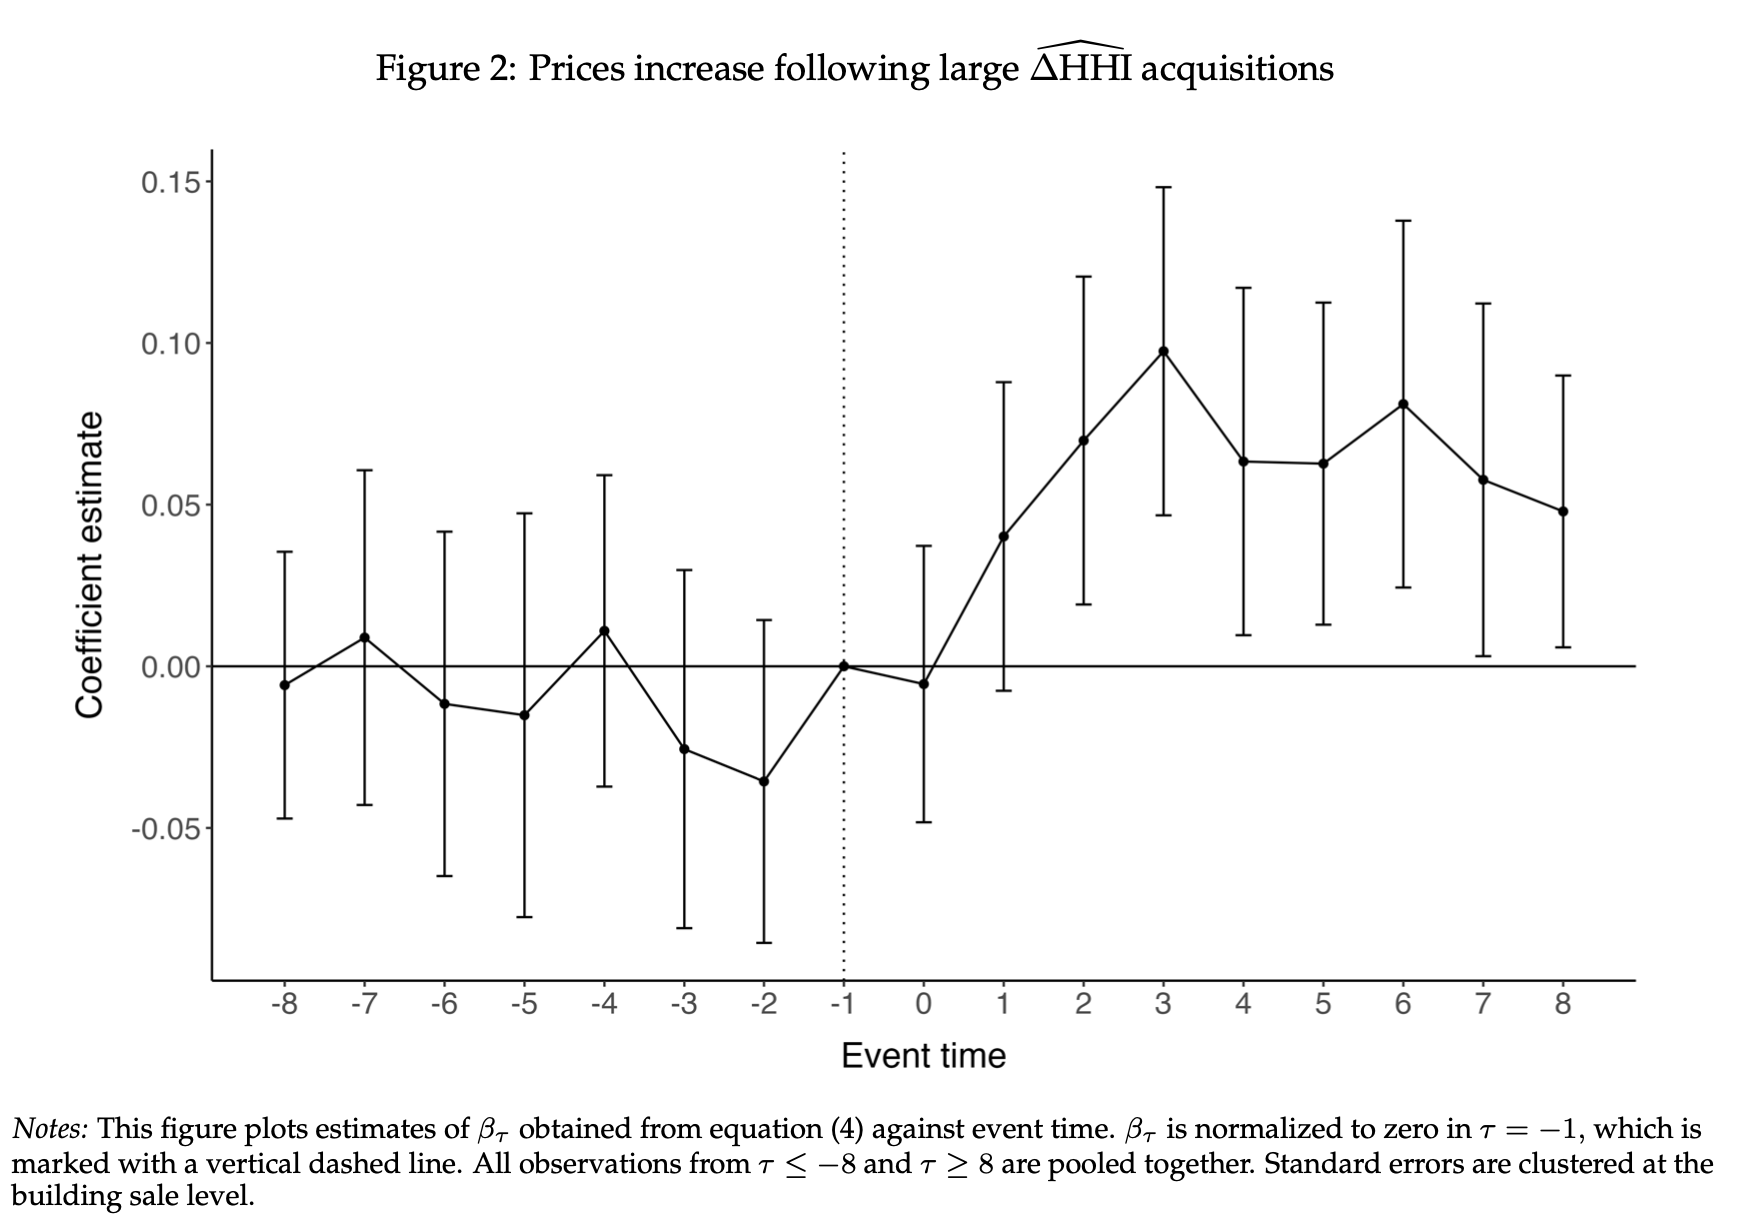
\includegraphics[width=0.5\linewidth]{figs/fern-jmp-prices.png}
        \caption{Effect of large merger on prices}
        \label{fig:fern-prices}
    \end{figure}
    \hyperlink{slide:searchmotivation}{\beamergotobutton{Search }}
\end{frame}

\begin{frame}{Motivating the Search Model}\label{slide:fern-vacancies}
Consistent with model of quantity restriction, when there is a large merger, the merging landlord reduces vacancies by about 0.2-0.4 \textit{units} (about a ~5-10\% reduction in own supply)
    \begin{figure}
        \centering
        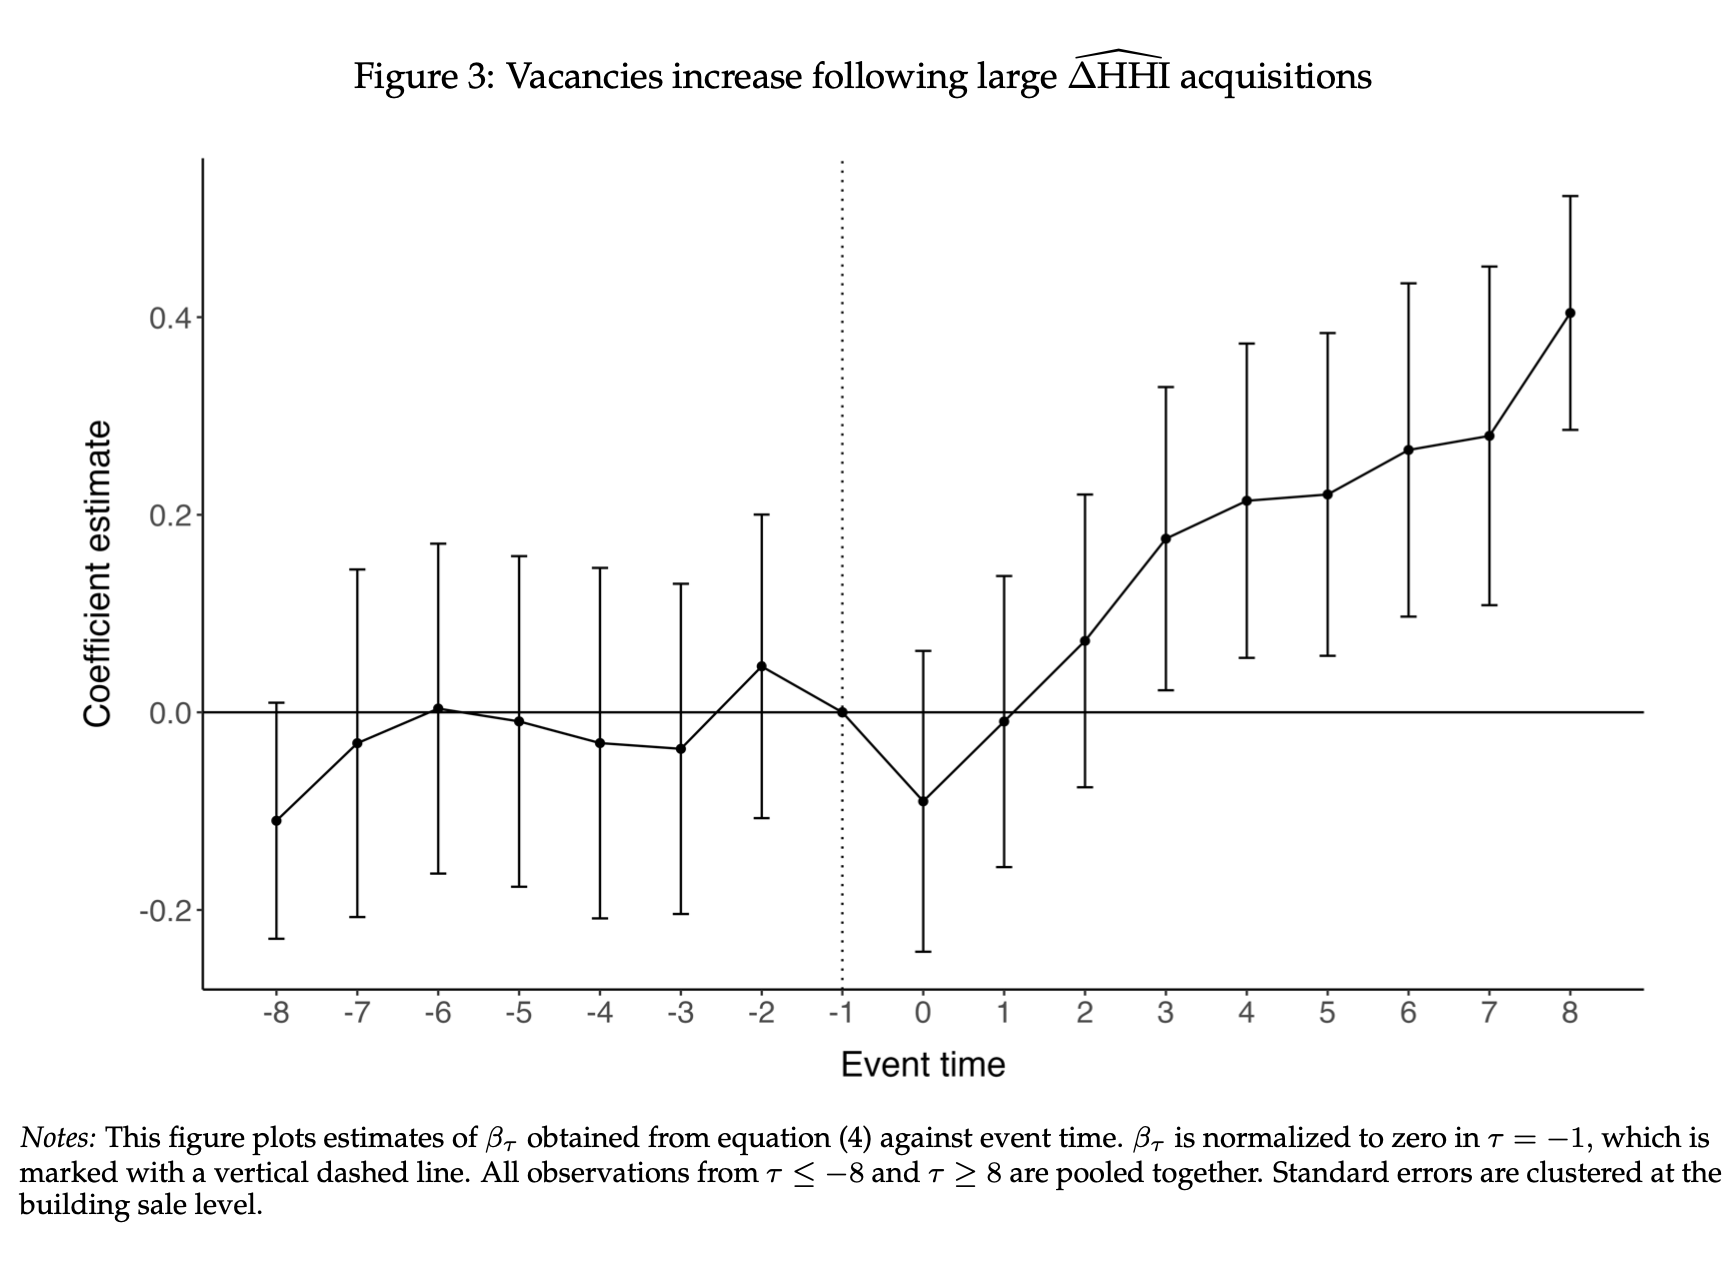
\includegraphics[width=0.5\linewidth]{figs/fern-jmp-vacancy.png}
        \caption{Effect of large merger on vacancies}
        \label{fig:fern-vacancies}
    \end{figure}
    \hyperlink{slide:searchmotivation}{\beamergotobutton{Search }}
\end{frame}





\end{document}
